\documentclass{beamer}

\usepackage{amsmath}
\usepackage{float}
\usepackage{graphicx}
\usepackage{caption}
\usepackage{xeCJK}

\setCJKmainfont{WenQuanYi Zen Hei}

\begin{document}
\title{An Efficient Algorithm for State Propagation on Graph with Lockable Vertices}
\author{Yuxiang Lin(林宇翔)}
\date{}

\begin{frame}
	\titlepage
\end{frame}

\begin{frame}
	\frametitle{Introduction}
\end{frame}

\begin{frame}
	\frametitle{Example}
	\begin{figure}
		\centering
		\includegraphics[width=0.5\textwidth,angle=-90]{../paper/graph/example/0.eps}
		\caption{$ \mathrm{set}(0, \mathit{true}) $}
	\end{figure}
\end{frame}

\begin{frame}
	\frametitle{Example}
	\begin{figure}
		\centering
		\includegraphics[width=0.5\textwidth,angle=-90]{../paper/graph/example/1.eps}
		\caption{$ \mathrm{setLock}(5, \mathit{true}) $}
	\end{figure}
\end{frame}

\begin{frame}
	\frametitle{Example}
	\begin{figure}
		\centering
		\includegraphics[width=0.5\textwidth,angle=-90]{../paper/graph/example/2.eps}
		\caption{$ \mathrm{propagate}() $}
	\end{figure}
\end{frame}

\begin{frame}
	\frametitle{Example}
	\begin{figure}
		\centering
		\includegraphics[width=0.5\textwidth,angle=-90]{../paper/graph/example/3.eps}
		\caption{$ \mathrm{setLock}(5, \mathit{false}) $}
	\end{figure}
\end{frame}

\begin{frame}
	\frametitle{Example}
	\begin{figure}
		\centering
		\includegraphics[width=0.5\textwidth,angle=-90]{../paper/graph/example/4.eps}
		\caption{$ \mathrm{setLock}(3, \mathit{true}) $}
	\end{figure}
\end{frame}

\begin{frame}
	\frametitle{Example}
	\begin{figure}
		\centering
		\includegraphics[width=0.5\textwidth,angle=-90]{../paper/graph/example/5.eps}
		\caption{$ \mathrm{propagate}() $}
	\end{figure}
\end{frame}

\begin{frame}
	\frametitle{The Algorithm}
	\begin{table}
	\tiny
	\centering
	\begin{tabular}{|l|l|l|}
		\hline
					 & $ \mathrm{set}() $ and $ \mathrm{setLock}() $ & $ \mathrm{propagate}() $                                \\ \hline
		small vertex & notify all large neighbors                    & iterate through all neighbors                           \\ \hline
		large vertex & notify all large neighbors                    & iterate through queues of potential sources and targets \\ \hline
	\end{tabular}
	\caption{Vertex interaction with neighbors when being acted on.}
	\end{table}

	\begin{center}
	Total time complexity: $ O\left(\lvert V \rvert + q \sqrt{\lvert E \rvert} \right) $
	\end{center}
\end{frame}

\begin{frame}
	\frametitle{Experiments}
	\begin{figure}
		\centering
		\includegraphics[width=0.5\textwidth,angle=-90]{../paper/graph/ba_q_1000000_10_0.1_power_3.eps}
		\caption{Time in seconds after executing $ q $ operations on $ G_\mathrm{BA}(10^6, 10), w_v = \mathit{deg}_v^3 $}
	\end{figure}
\end{frame}

\begin{frame}
	\frametitle{Applications}
	\begin{itemize}
		\item Machine learning.
		\item Information transmission on social networks.
		\item Modelling the spreading of disease.
	\end{itemize}
\end{frame}

\begin{frame}
	\begin{center}
	{\Huge Thanks for watching!}
	\end{center}
\end{frame}

\end{document}
